\documentclass{beamer}
\usepackage{graphicx}

\title{Visualisation des donn\'ees multivari\'ees avec lattice}
\author{Toby Dylan Hocking}

\AtBeginSection[]
{
  \begin{frame}<beamer>
    \frametitle{Outline}
    \tableofcontents[currentsection]
  \end{frame}
}

\AtBeginSubsection[]
{
  \begin{frame}<beamer>
    \frametitle{Outline}
    \tableofcontents[currentsection,currentsubsection]
  \end{frame}
}

\frame{\titlepage}

\newcommand{\framet}[2]{\frame{
\begin{itemize}
\frametitle{#1}{#2}
\end{itemize}
}}

\newcommand{\picframe}[1]{
  \frame[plain]{
    \includegraphics[width=\textwidth]{#1}
  }
}

\begin{document}

\section{lattice}

\section{latticeExtra}

\section{latticedl}

\framet{Direct labels are almost always better than legends}{
Edward Tufte, professor emeritus of Statistics at Yale
1983, The Visual Display of Quantitative Information
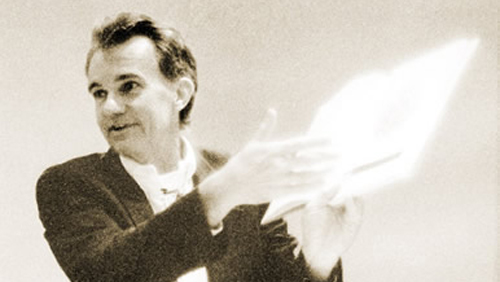
\includegraphics{TUFTE}
}
